\chapter{Design \& Implementation}\label{sec:impl}

\section{Bitwidth analysis}
The analysis is a data flow analysis. The analysis attaches an $(int,boolean)$ tuple to every meaningful node. A node is considered meaningful if the node has an integer-mode. We will reference the first value as \emph{stable bits} and the second bit as \emph{is positive}. \newline
What stable here means can be observed when looking at \ref{fig:numbers}.
For the first line of the table we have five stable digits. The second line has 7 stable digits.\newline
Since this is a data flow analysis, which is built on an iterative approach. We might want to address the current tuple of a node $x$, while we have a new one calculated. Therefore we call $\hat{x}$ the currently associated value, and $x$ the newly calculated one.

\paragraph{Bit representation}
The stable bits indicate how many bits are stable, and therefore not used.
The second value of the tuple indicates if the value will ever reach negative numbers or not. Thus it indicates at least one stable bit at the highest position. However, the second value is only meaningful for modes that allow signs.

\paragraph{Range representation}
There is also a second way of interpreting the two values. The stable bits can define a minimum and maximum range. The maximum number is reached if the stable bits are all zero, and the rest one. If the mode is signed and the node is not positive, then the minimum number is reached by assuming all stable bits are one, and the rest zero. Otherwise the minimum is 0. We can define the following min max definitions for the ranges:

$
max_{bitwidth}(x)=
\left\{
\begin{array}{l}2^{stable\_digits-1}-1\\2^{stable\_digits}-1\end{array}
\begin{array}{l} {mode.signed} \\ {Otherwise} \end{array}
\right.
$

$
min_{bitwidth}(x)=
\left\{
\begin{array}{l}2^{stable\_digits-1}\\0\end{array}
\begin{array}{l} {mode.signed \wedge is\_positive} \\ {Otherwise} \end{array}
\right.
$

\begin{figure}
	\centering
	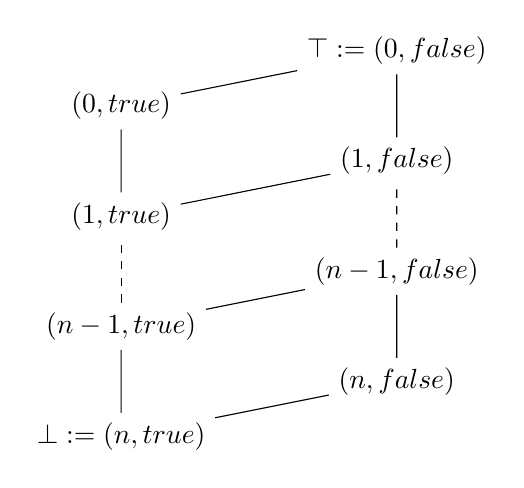
\begin{tikzpicture}[scale=.7]
		\node (np0) at(0,0) {$\bot := (n,true)$};
		\node (np1) at(0,2) {$(n-1,true)$};
		\node (np2) at(0,4) {$(1,true)$};
		\node (np3) at(0,6) {$(0,true)$};
		\node (p0) at(5,1) {$(n,false)$};
		\node (p1) at(5,3) {$(n-1,false)$};
		\node (p2) at(5,5) {$(1,false)$};
		\node (p3) at(5,7) {$\top := (0,false)$};
		\draw (np0) -- (p0) -- (p1) -- (np1) -- (np0);
		\draw (np2) -- (p2) -- (p3) -- (np3) -- (np2);
		\draw [dashed] (np1) -- (np2);
		\draw [dashed] (p1) -- (p2);
	\end{tikzpicture}
\caption{Hesse diagram of the lattice which is used in this analysis}
\label{fig:lattice}
\end{figure}

\paragraph{Analysis} The analysis works as a fixed point iteration. Therefore we use  \autoref{fig:lattice} as lattice. The values of the lattice are representing the tuples from the analysis.

As a first step, we iterate over every single node and initialize the node with $\top$ and mark it as \textit{dirty}. If the node is constant, we calculate its bitwidth. Nodes with the opcodes \textit{Const}, \textit{Size} and \textit{Address} are considered constant.

The second step consists of recalculating every \textit{dirty} node in the graph. if the stable bits of $x$ are greater than those from $\hat{x}$, then the new value is memorized as $\hat{x}$ of the node and every successor of the node is marked as dirty. The used rules for recalculating the nodes are described in \autoref{table_of_rules}.

\subsection{Value prediction}
In addition to the normal analysis results, the fixed point iteration can insert additional 
confirm nodes. Those confirm nodes help making the analysis more accurate.
First of all we need a few definitions for easier understanding:

\subparagraph{Definition: True / false Blocks}
A compare node in \libFIRM has always a relation, 2 operands and 2 blocks. One of the blocks is executed depending on if the criteria was meet or not. The block that is executed when it was meet, is called \emph{true-block} the other block is called \emph{false-block}. The structure is visualized in \autoref{fig:compare_upper_bound}
\begin{figure}
	\centering
	\begin{tikzpicture}[scale=1.0, transform shape]
	\node[graph]{
		\begin{tikzpicture}[remember picture]
		\node[block] (startblock) {
			\begin{tikzpicture}
			\node[firm]    (predessors)       at (-1,3) {$\omega$};
			\node[const]    (c2)       at ( 1,3) {Const X};
			\node[firm]    (cmp)        at ( 0,2) {Cmp};
			\node[control] (cond)       at ( 0,1) {Cond};
			\node[control] (false)      at (-1,0) {False};
			\node[control] (true)       at ( 1,0) {True};
			
			\draw[dataDependency]    (cmp.120)     -- ++(0,0.1) -| (predessors);
			\draw[dataDependency]    (cmp.60)      -- ++(0,0.1) -| (c2);
			\draw[dataDependency]    (cond)        --              (cmp);
			\draw[controlDependency] (false.north) -- ++(0,0.1) -| (cond.240);
			\draw[controlDependency] (true.north)  -- ++(0,0.1) -| (cond.300);
			\end{tikzpicture}
		};
		\node[block, anchor=north east] (left) at ($(startblock.south) + (-1,-0.5)$) {
			\begin{tikzpicture}
			\node[const] (c0) at (0,0) {$\ominus$};
			\end{tikzpicture}
		};
		\node[block, anchor=north west] (right) at ($(startblock.south) + (1,-0.5)$) {
			\begin{tikzpicture}
			\node[const] (c1) at (0,0) {$\iota$};
			\end{tikzpicture}
		};		
		% Control dependencies
		\begin{scope}[every path/.style = {controlDependency}]
			\draw (left.north)  -- ++(0,0.2) -| (false);
			\draw (right.north) -- ++(0,0.2) -| (true);
		\end{scope}
		
	\end{tikzpicture}
};
\end{tikzpicture}
\caption{The definition of a upper bound compare node}
\label{fig:compare_upper_bound}
\end{figure}


\subparagraph{Definition: Upper bounds}
A node defines a upper bound if the relation is < and the second operand is constant.\newline
A compare node is also defining a upper bound if it can be transformed into a construct that matches the definition. For example by switching the right and left nodes, while turning the relation.

\subparagraph{Definition: Predecessor in a certain block}
In the detection described later, we often need to find a predecessor that is placed in a certain block. Therefore we define:
\begin{center}
$\kappa(a, b) := \{X| X \leftarrow a \wedge X.block = b \}$ 
\end{center}

It will return every node that is located in \textit{b} and is a predecessor of \textit{a}.

\subparagraph{Definition: Constant dependencies}
\begin{figure}
	\centering
	\begin{tikzpicture}
		\node[graph]{
			\begin{tikzpicture}[remember picture]
				\node[block] (startblock) {
					\begin{tikzpicture}


						\node[firm]    (const1) at (3,3) {Const};
						\node[firm]    (const2) at (3,2) {Const};
						\node[firm]    (mul)    at (1,2) {Mul};
						\node[firm]    (add)    at (1,1) {Add};
						\node[firm]    (sub)    at (0,0) {Sub := $\lambda$};
						\node[firm]    (mul2)    at (-0.5,3) {Mul};
						\node[firm]    (mod)    at (1,3) {Mod};

						\draw[dataDependency]    (sub.60)      -- ++(0,0.1) -| (add);
						\draw[dataDependency]    (sub.north)   -- ++(0,0.1) -| (mul2);	
						\draw[dataDependency]    (add.north)     -- ++(0,0.1) -| (mul);
						\draw[dataDependency]    (add.60)      -- ++(0,0.1) -| (const2);
						\draw[dataDependency]    (mul.60)     -- ++(0,0.1) -| (const1);
						\draw[dataDependency]    (mul.north)   -- ++(0,0.1) -| (mod);
						
						\draw[red, thick,dotted]     ($(mul.north west)+(-0.15,0.15)$) rectangle ($(add.south east)+(0.15,-0.15)$);
					\end{tikzpicture}
				};
			\end{tikzpicture}
		};
	\end{tikzpicture}
    %FIXME highlight mul and addli
\caption{A subgraph of a FIRM graph. The result of $\xi(\lambda)$ is highlighted in red}
\label{fig:def:xi}
\end{figure}
While looking at C code we often see that addition and multiplication nodes are used for calculating array addresses or addresses for structure access. Therefore one operant of the arithmetical operations is often constant. A example for this can be found at \autoref{fig:def:xi}.
We define $\xi$ to explore the whole tree of one constant one not constant operants, and return us every node that was not constant.
\begin{center}
$\xi(a) := 
\left\{
	\begin{array}{l}
		a \cup \xi(c)\\ 
		\emptyset
	\end{array}
	\begin{array}{l}
		, \text{If there is only one not constant dependency \textit{c}} \\ 
		, \text{otherwise}.
	\end{array}
\right.$
\end{center}

If \textit{a} has only one not constant operant c, then $\xi$ returns the element a and $\xi(c)$. Otherwise it returns a empty set. For the example the highlighted nodes will be part of $\xi(Y)$.

\paragraph{Upper bounds for block execution}
The values that are calculated in a node are (even if the fixed point iteration is not stable yet) possible values. The iteration starts at $\bot$ and moves into the direction of $\top$. 
%This means for a node \textit{n} our range of possible values starts at something like $[0,0]$, moving towards $[max _{bitwidth}(n), min _{bitwidth}(n)]$ with each iteration.  %CORRECTION LINE
We now evaluate a upper bound compare node, every time the first operand changes. In the beginning we can say that that with those possible values, each time the true-block will be executed. However, if $max _{bitwidth}(n)$ grows enough to get bigger than the second operand or the compare node, then we can say that we have found a upper bound for the execution of the true-block. Which is $max _{bitwidth}(n)$ in the current state. Thus we can insert a confirm node between every node $e \in \kappa(i, j)$ and $i$. Where $i$ is the first operand and j is the true block.

\paragraph{Extended confirm insertion}
The confirm nodes that we have inserted in the paragraph before can also be transported backwards.
With $\xi(i)$ we can get a set of nodes, where the current state in the analysis is only depending on one node. Thus we can say that the state of every node from $\xi(i)$ will not change as long as the most upper element in the tree structure does not change. Which means that we can for every $e \in \xi(i)$ and $g \in \kappa(e, j)$ insert a confirm node between $(e,g)$

\section{Stable Conversion nodes}
In libfirm a conversion node can be used to convert one dataword from one mode to another. This type of node has one operand. Such a conversion has two effects. The bitwise representation stays the same. Or the bitwise representation changes, due to the numerical representation changes. We call the first case \textit{Stable Conversion node}.  A example for a unstable conversion node may look like $(unsigned)((int)-10)$. A stable conversion node might look like $(unsigned)(int)10$.

\paragraph{Finding stable conversion nodes}
Such stable conversion nodes can be found using the bitwidth analysis. We compare the range from the operand with the range from the conversion node itself. If the ranges are the same, then we know that the conversion is stable.

\paragraph{Removing conversion nodes}
\begin{figure}
	\centering
	\begin{tikzpicture}[scale=.7]
		\node[graph]{
			\begin{tikzpicture}[remember picture]
				\node[block] (startblock) {
					\begin{tikzpicture}
					
					
					\node[firm]    (conv) at (-1,2) {Conv};
					\node[firm]    (const) at (1,2) {Const};
					\node[firm]    (cmp)    at (0,1) {Cmp};
					\node[firm]    (cond)    at (0,0) {Cond};

					\draw[dataDependency]    (conv.north)   -- ++(0,0) -| (-1,3);	
					
					\draw[dataDependency]    (cmp.60)      -- ++(0,0.1) -| (const);
					\draw[dataDependency]    (cmp.120)      -- ++(0,0.1) -| (conv);
					\draw[dataDependency]    (cond.north)     -- ++(0,0.1) -| (cmp.south);
					
					\end{tikzpicture}
				};
			\end{tikzpicture}
		};
	\end{tikzpicture}
\caption{Conversion compare construction}
\label{fig:example:conversion_opt}
\end{figure}
In case we found a stable conversion node, then we can say that this node only exists for syntax rules, there is no semantical value in them. Removing those nodes also has the advantage of helping other analyses. The confirm insertion algorithm of libfirm is searching for assertions that can be made based on looking at compare nodes. This works quite well. However, the example at \autoref{fig:example:conversion_opt} does not work
The insertion code could only insert a Confirm between the Compare and the conversion. However, it would need to be behind the conversion node, in order to help the rest of the code, since other nodes will likely depend on the operand of the conversion node and not on the conversion node itself. 
After removing the conversion node, the analysis can find a assertion based on the compare node. This also helps the branch prediction and dead code elimination.

However, for really removing the conversion nodes, we need to find situations where we can eliminate the conversion node. We have already seen the example with a compare node. Additionally we can do the same with a arithmetical operation.

\paragraph{Compare-Conversion optimization}
There is the rule in libfirm that the two operands of a compare node are forced to have the same mode. This means, when we remove the conversion node, we also need to adjust the mode of the second operand. This is not easily possible for something that is not a constant, thus we confine for now that the two operands need to be a conversion and a constant node.
With the assertion that our second operand is a constant, we can simply adjust its mode. And remove the conversion. 

\paragraph{Arithmetical-Conversion optimization}
\begin{figure}
	\centering
	\begin{tikzpicture}[scale=.7]
		\node[inner sep=0pt] (russell) at (0,0){
			\includegraphics[width=.25\textwidth]{fig/arithmetical_opt.png}
		};
	\end{tikzpicture}
\caption{Arithmetical optimization example}
\label{fig:example:arithmetical_opt}
\end{figure}
A other situation where we can optimize the conversion nodes are arithmetical operations, where one operand is again constant. In this case we don't really remove the conversion node, we more drag it through the arithmetical operation, and place it afterwards. We do this and hope that we can remove it with a compare conversion optimization after that.
Such a construct might look like \autoref{fig:example:arithmetical_opt} . After we adjusted the mode of the constant we can move the conversion from the operand of the arithmetical operation to the end.
\section{VHDL generation}
Projects like libva have made the first step into the direction of hardware accelated video decoding on a computer system. The projects tries to provide standardized access to the for decoding video streams like MPEG-2, H.264/AVC, H.265/HEVC, VP8, VP9, VC-1. The project itself handles the passing and messaging from a front end application like a video player, to the driver itself. The driver itself then answers the calls from the API. And the decoded picture goes back to the front end application. However, the driver itself still needs to do the decoding on its side. Preferable implemented in hardware, since this is usually providing the best performance. The amount of work needed for implementing such a decoder for MPEG-2 can be found in \cite{mpeg2-modelling}. %a63b48fa89cc2a673e4899c174459bc2e290.pdf
While looking at this it seems like a good idea to think about writing the code in a higher level language and let it simply compile against vhdl. Exactly this is done by the firm tool \textit{firm2vhdl}.
\paragraph{firm2vhdl} The tool provides the transformation from a libfirm graph into vhdl code. Every node in the firm graph gets transformed into a instruction in vhdl. This is done in done by calculating the effect the node has in vhdl code, by using its operands, assigning the result to a new variable. Which then can be used again later by the next operation. 
Each of those those variables are represented in hardware, and thus have a amount of bits. Which is, at this state, the number of bits of the mode.

\paragraph{bitwidth in firm2vhdl}
Using the number of bits for a bit can be very wasteful in vhdl as this is wasting a lot of space on the FPGA chip later on. Minimizing the amount of bits used per variable here can be important, since most of the variables used in c are not using the complete bandwidth.\newline
The bitwidth information gathered from the analysis described before can help here, as it defines how many bits of a node are used, and how many are not. Thus we can add code to the transformation, for taking the used bits, instead of the number of bits in a mode.

\section{How about section}
This section is about decisions that where made, and why they are made.

\subsection{Value range vs. bitwidth}

%Where is the actaul difference when looking at the rules.
The analysis previously explained is outputting bitwidth informations. The fixpoint iteration uses the set of rules described in \autoref{table_of_rules}. The same analysis could use a set of rules where we don't calculate the bitwidth, but rather the direct range of possible values (Not bound to $2^x$ form). There is already such a implementation in \libFIRM, its called value range propagation (VRP).

%What are the costs for jumping one bit further
However, there should be some way to compare both models. We know that every node in libfirm has a mode, this mode is defining the length of a data word. The analysis is measuring how many of the bits from this data word are used. So once a node gets marked dirty, there is some sort of delta, like $ \delta = max _{bitwidth}(\textsc{}x) - max _{bitwidth}(\hat{x}) $.
In case of bitwidth, we know that the delta will have the form of $2^x$. In case of the value range detection, the only assertion we can have is $\delta = 1$.
Now lets take a graph like ???, where X is some sub graph that performs a operation. Under the assertion that the delta of last node is minimal, then the bitwidth analysis is faster.
A real life example where this is happening is for example the simple access to a array, like $array[i]$.
%Sample run on a for / while loop



\subsection{Widening \& Narrowing}
%what is widening / narrowing
%The idea of widening and narrowing is, that you can make your optimization 

%How are graphs looking like in real world, where is the worst case when comparing vrp to bwa

%Why is there no big difference between the results of the vrp and the bwa

